\documentclass[tikz,border=3.14mm]{standalone}

% colors
\definecolor{mylightred}{RGB}{255,210,210}
\definecolor{myred}{RGB}{200,100,100}
\definecolor{mydarkred}{RGB}{140,40,40}
\definecolor{mylightblue}{RGB}{220,228,255}
\definecolor{myblue}{RGB}{183,191,229}
\definecolor{mydarkblue}{RGB}{50,70,190}
\definecolor{brass}{rgb}{0.71, 0.65, 0.26}

\begin{document}

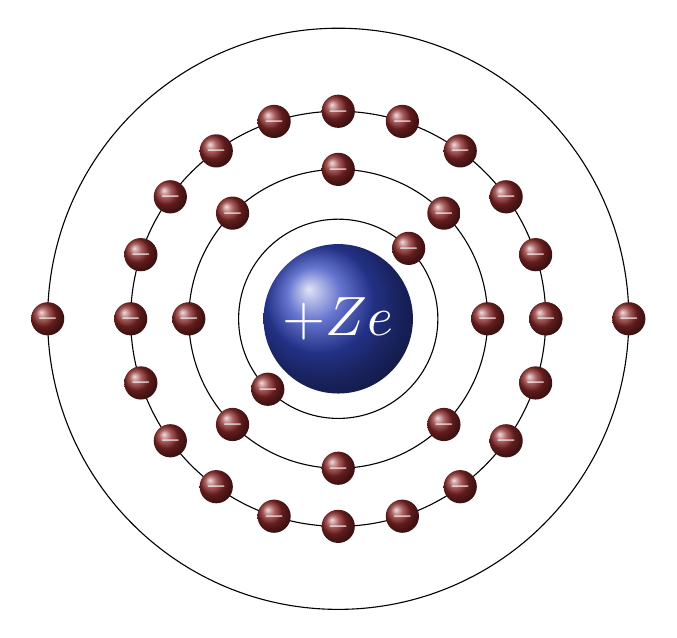
\begin{tikzpicture}[scale=3]
\def\e{$-$}
\def\pi{3.141592}
\def\ra{12pt}
\def\rb{18pt}
\def\rc{25pt}
\def\rd{35pt}
  \coordinate (O)  at (0,0);
  \shade[radius=9pt,ball color = mydarkblue,align=center] (O) circle node[scale=2.0,white] {$+Ze$};
  \draw[black]            (O) circle (\ra);
  \foreach \theta in {\pi/4,5*\pi/4}
    {
     \shade[radius=2.0pt,ball color = mydarkred]  ({\ra*cos(\theta r)}, {\ra*sin(\theta r)})  circle node[scale=1.0,white] {\e};
    }
  \draw[black]            (O) circle (\rb);
  \foreach \theta in {0,2*\pi/8,2*\pi/4,2*3*\pi/8,2*\pi/2,2*5*\pi/8,2*3*\pi/4,2*7*\pi/8}
    {
     \shade[radius=2.0pt,ball color =mydarkred]  ({\rb*cos(\theta r)}, {\rb*sin(\theta r)})  circle node[scale=1.0,white] {\e};
    }
  \draw[black]            (O) circle (\rc);
  \foreach \theta in {0,1,...,20}
    {
     \shade[radius=2.0pt,ball color =mydarkred]  ({\rc*cos(2*\theta*\pi/20 r)}, {\rc*sin(2*\theta*\pi/20 r)})  circle node[scale=1.0,white] {\e};
    }
  \draw[black]            (O) circle (\rd);
  \foreach \theta in {0,1}
    {
     \shade[radius=2.0pt,ball color = mydarkred]  ({\rd*cos(\theta*\pi r)}, {\rd*sin(\theta*\pi r)})  circle node[scale=1.0,white] {\e};
    }
\end{tikzpicture}
\end{document}